\documentclass{article}

\usepackage{listings}
\usepackage{amsmath}
\usepackage{graphicx}
\usepackage{hyperref}
\usepackage{booktabs}
\usepackage{verbatim}
\usepackage{url}
\usepackage{framed}
\usepackage{booktabs}

\begin{document}

\title{Homework 12}
\author{Geoffrey Ulman\\
        CSI740}
\date{April 2012}
\maketitle

\section{Problem 1}\label{p1}

The power iteration algorithm was implemented as specified in Algorithm 27.1 with the rate of change in the calculated eigenvalue used as a stopping condition. All calculations were run until the rate of change dropped below \(10^{-8}\).

Figures \ref{p1t1} and \ref{p1f1} summarize the convergence rate of the power iteration algoirhtm on the \(A\) matrix for a random initialization vector. Figure \ref{p1f1} plots the difference between the actual largest eigenvalue (as calculated by Matlab's \verb|eig| command) and the calculated eigenvalue on a log scale. Because the trend appears linear on the log scale, the convergence rate appears to be exponential.

Figure \ref{p1f2} plots the \(R_m\) ratio at each iteration. The blue line indicates the square of the ratio between the true second-largest and largest eigenvalues of \(A\) as calculated by Matlab's \verb|eig| command. As expected, these values agree quite well.

Finally, Figure \ref{p1f3} summarizes the number of iterations necessary to meet the stopping criteria for 1000 runs of the power iteration algorithm, each with a different random initial vector. A small number of initial vectors required one additional or one less iteration to converge. However, in general the choice of initial vector has little to no impact on the convergence rate. Of course, if a degenerate vector is chosen, like the zero vector or one of the other eigenvectors of \(A\), then the algorithm may fail.

\begin{figure}
\centering
\begin{tabular}{lrr}
\toprule
Iteration & Eigenvalue & Error \\
\midrule
 1 & 332.7815351291716 & 0.064780277883358 \\
 2 & 332.8461979585259 & 0.000117448529011 \\
 3 & 332.8463151514994 & 0.000000255555506 \\
 4 & 332.8463154064969 & 0.000000000558032 \\
 5 & 332.8463154070536 & 0.000000000001307 \\
 6 & 332.8463154070549 & 0.000000000000057 \\
\bottomrule
\label{p1t1}
\end{tabular}
\caption{Power Iteration: Error in Calculated Eigenvalue by Iteration}
\end{figure}

\begin{figure}
\centering
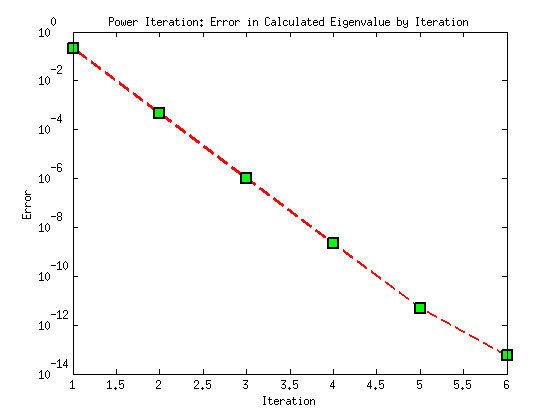
\includegraphics[width=0.8\textwidth]{Problem1Figure1.png}
\caption{Power Iteration: Error in Calculated Eigenvalue by Iteration}
\label{p1f1}
\end{figure}

\begin{figure}
\centering
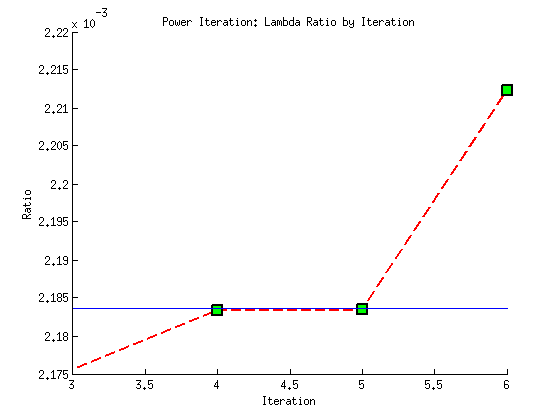
\includegraphics[width=0.8\textwidth]{Problem1Figure2.png}
\caption{Power Iteration: Lambda Ratio by Iteration}
\label{p1f2}
\end{figure}

\begin{figure}
\centering
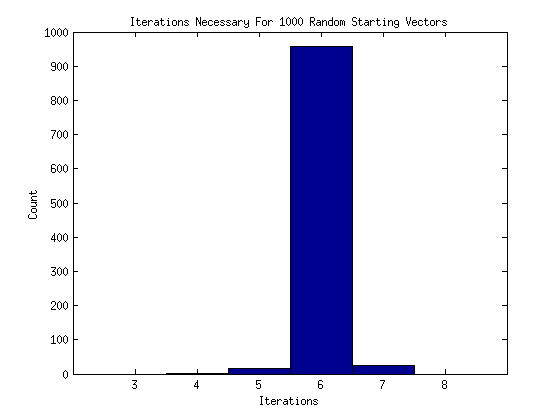
\includegraphics[width=0.8\textwidth]{Problem1Figure3.png}
\caption{Power Iteration: Iterations Necessary for 1000 Random Starting Vectors}
\label{p1f3}
\end{figure}

\end{document}
